\documentclass[10pt,graphicx,caption,rotating]{article}
\textheight=24cm
\textwidth=18cm
\topmargin=-2cm
\oddsidemargin=0cm
\usepackage[utf8x]{inputenc}
\usepackage[activeacute,spanish]{babel}
\usepackage{amssymb,amsfonts}
\usepackage[tbtags]{amsmath}
%7\usepackage{slashbox}
\usepackage{pict2e}
\usepackage{float}
\usepackage[all]{xy}
\usepackage{graphics,graphicx,color,colortbl}
\usepackage{times}
\usepackage{subfigure}
\usepackage{wrapfig}
\usepackage{multicol}
\usepackage{colortbl}
\usepackage{cite}
\usepackage{url}
\usepackage[tbtags]{amsmath}
\usepackage{amsmath,amssymb,amsfonts,amsbsy}
\usepackage{bm}
\usepackage{algorithm}
\usepackage{algorithmic}
\usepackage[centerlast, small]{caption}
\usepackage[colorlinks=true, citecolor=blue, linkcolor=blue, urlcolor=blue,
breaklinks=true]{hyperref}

\title{Tarea 1 - Introducción a los sistemas de control}

\author{David Ricardo Martínez Hernández}
\date{}
\begin{document}
\maketitle

\section{Estructura jerárquica de automatización}
\noindent
INFINEON Technologies AG\\
\noindent
Empresa alemana de fabricación de semiconductores y sistemas de automatización. Surgió en 1999 como parte de la separación del área de manufactura de semiconductores de Siemens AG, la empresa madre. En 2010 la empresa contaba con más de 25000 empleados a nivel mundial ofreciendo todo tipo de servicios en el área de la automatización\footnote{Tomado de \cite{page1}}.\\
Actualmente la empresa se desenvuelve en tres campos de acción:
\begin{itemize}
  \item \textbf{Automática:} proveedor de chips y tarjetas impresas para uso en el control de motores y transmisiones (microcontroladores, semiconductores de potencia y sensores), electrónica para el comfort y la seguridad (Airbags, frenos ABS, Electronic Stability Control).
  \item \textbf{Industrial y Multimercado:} Semiconductores de potencia para uso en actividades de generación, transmisión y consumo de energía eléctrica. Aplicaciones que van desde control de accionamientos para sistemas de potencia (electric drives), hasta electrodomésticos, módulos de energías renovables, semiconductores para módulos de iluminación y tecnología LED, fuentes de poder para Pcs, electrónica de consumo, aplicaciones médicas, dispositivos de alta frecuencia, entre otros.
  \item \textbf{Circuitos Impresos y Seguridad:} Microcontroladores para tarjetas SIM de telefonía celular, tarjetas bancarias y dispositivos electrónicos RFID para identificación de pasaportes y documentos oficiales.
\end{itemize}
Visión de la empresa en cuanto a automatización, según su brochure\footnote{Tomado de \cite{page2}}:
\begin{figure}[H]
	\centering
		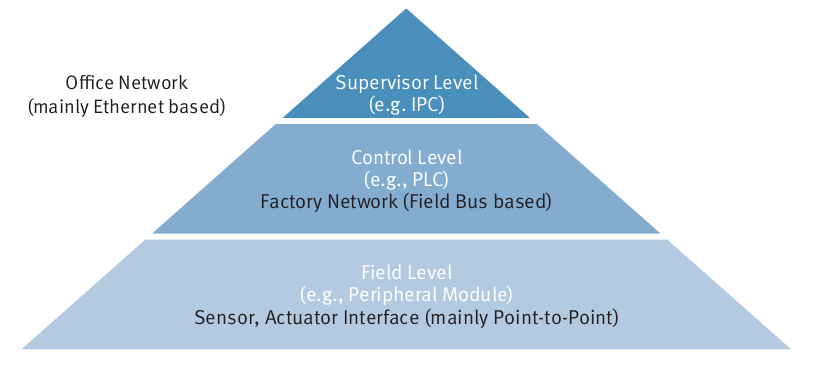
\includegraphics[scale=0.5]{image1.png}
	\caption{Visión Empresa (Tomado de \cite{page2}).}
	\label{fig1}
\end{figure}
En cada nivel desarrollan un resumen de las unidades mayoritariamente involucradas en él, como se muestra a continuación:
\begin{figure}[H]
	\centering
		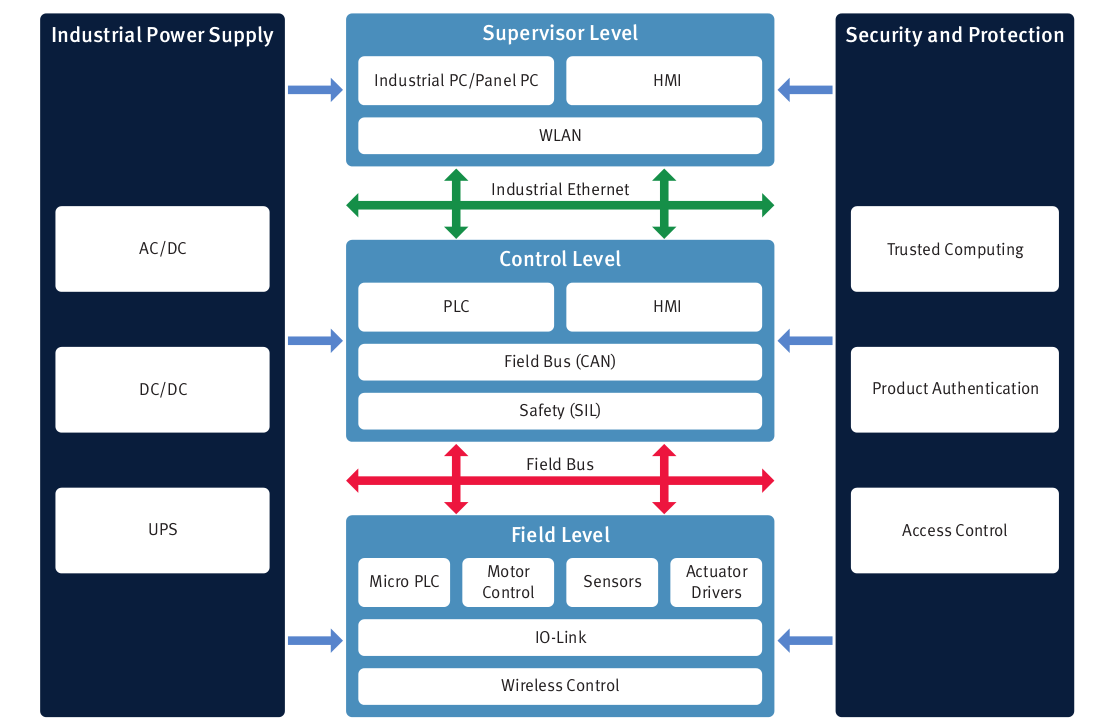
\includegraphics[scale=0.4]{image2.png}
	\caption{Niveles (Tomado de \cite{page2}).}
	\label{fig2}
\end{figure}

\begin{itemize}
  \item \textbf{Nivel Supervisorio:} Sistemas basados en procesamiento por computador. (industrial PC, en forma de computadoras personales, racks y “Panel Pcs”) Equipados con sistema operativo Windows embebido, y software específico para control y visualización. Estos sistemas generalmente están interconectados en una red Gigabit LAN (o WLAN) o alguna otra de banda ancha, que permite visualizar información a nivel corporatio. Estos sistemas no poseen altas especificaciones de respuesta temporal, esta tarea recae en dispositivos del nivel de control. No contiene ninguna arquitectura de control. Como protección de datos, posee redundancia en las unidades de energía de los sistemas (UPSs)
  \begin{itemize}
    \item \textbf{Industrial PC (IPC):} Sistemas basados en software, que cumplen con requerimientos de operación en campo, como protección, consumo eficiente de energía, compatibilidad de software, sistemas de comunicación, etc.
    \item \textbf{Human Machine Interface (HMI):} displays de texto, gráficas, mímicos, panel Pcs, etc. Tienen como objetivo ser lo más simples e ilustrativos posibles, tal que el operario los encuentre cómodos para su monitoreo.
    \item \textbf{Wireless Local Area Network (WLAN):} Filtros de ruido y amplificadores de señal que permiten extender el alcance de alguna comunicación.
  \end{itemize}
  \item \textbf{Nivel de Control:} Sistemas de automatización (PLCs principalmente). Poseen gran capacidad de reacción en tiempo real (isochronous real-time Ethernet), y un sistema operativo propio en el cual está construida la arquitectura de control. Posee protocolos de comunicación altamente eficientes (comunicaciones instantáneas). Estructura de PLCs modular y personalizable. Control de periféricos  comunicados por Fieldbus (algunos con un pre-procesamiento de datos).
  \begin{itemize}
    \item \textbf{Programable Logic Controller:} posee alta confiabilidad, protección e inmunidad contra ruido e influencias externas (algunos, con protección contra el medio en el que operan: agua y polvo). Operación continua y en un rango amplio de temperaturas, y seguridad de la información procesada.
    \item \textbf{HMI:} Necesario para la visualización de los datos recogidos por los sensores.
    \item \textbf{Controller Area Network (CAN bus)} como bus de campo ofrecido.
  \end{itemize}
  \item \textbf{Nivel de Campo:} Equipos terminales: sensores y actuadores, que en conjunto con unidades PLC o sistemas I/O remotos, realizan una captación de datos y un pre-procesamiento de la información adquirida. Usualmente conección punto-a-punto. Algunas aplicaciones donde no se requiere de interconexión con el sistema de control global, se usan microPLCs para ejecutar tareas individuales en campo.
  \begin{itemize}
    \item \textbf{Micro PLC. Aplicaciones sencillas (low-end apps):} domésticas o de electrónica comercial, donde el objetivo es que sea económico, sencillo de usar, tamaño reducido y altamente eficiente en uso de energía
    \item \textbf{Control de motores y accionamientos:} Tarjetas de control de los accionamientos (drives) de motores, desde brushless DC hasta motores de inducción y SRM.
    \item \textbf{Sensores: De alta precisión y rápida transferencia de datos:} Sensores inteligentes, de medición sin contacto, a base de semiconductores.
    \item \textbf{Actuadores de los accionamientos:} Semiconductores de potencia para controlar cargas inductivas de gran capacidad.
    \item \textbf{IO-Link:} Estándar de comunicaciones sencillo.
  \end{itemize}
\end{itemize}

\section[Siglas]{Términos frecuentes en Automatización y control de Procesos}
\begin{enumerate}
 \item \textbf{CIM (Computer-Integrated Manufacturing) Manufactura integrada por computadora:} Método de producción completamente controlado por computadora. Es el enfoque de fabricación a utilizar ordenadores para controlar el proceso de producción, se basa en los procesos de control en bucle cerrado\footnote{Tomado de \cite{page3}}.

 \item \textbf{CNC (Computer Numerical Control) Control Numérico por Computadora:} Es un sistema de automatización de máquinas que son operadas mediante comandos programados en un medio de almacenamiento, en comparación con el mando manual mediante volantes o palancas.\footnote{Tomado de \cite{page4}}.

 \item \textbf{DCS (Distributed Control System) Sistema de Control Distribuido:} Es un sistema de control aplicado, proceso o cualquier tipo de sistema dinámico, en el que los elementos del tratamiento no son centrales en la localización, sino que se distribuyen a lo largo de todo el sistema con cada componente. Todo el sistema de los controladores está conectado mediante redes de comunicación y de monitorización\footnote{Tomado de \cite{page5}}.

 \item \textbf{ERP (Enterprise Resource Planning) Planeación de Recursos Empresariales:} Son Sistemas de Información Gerenciales que integran y manejan muchos de los negocios asociados con las operaciones de producción y de los aspectos de distribución de una compañía en la producción de bienes o servicios\footnote{Tomado de \cite{page6}}.

 \item \textbf{HMI (Human-Machine Interface) Interfaz Usuario-Máquina:} Es el medio con que el usuario puede comunicarse con una máquina, un equipo o una computadora. Normalmente suelen ser fáciles de entender y fáciles de accionar. Incluyen elementos como menús, ventanas, teclado, ratón, los beeps y algunos otros sonidos que la computadora hace\footnote{Tomado de \cite{page7}}.

 \item \textbf{IEEE (Institute of Electrical and Electronics Engineers) Instituto de Ingenieros Eléctricos y Electrónicos:} \textit{``Es la asociación profesional más grande del mundo, dedicada al avance de la innovación tecnológica y la excelencia para el beneficio de la humanidad''}. Institución dedicada principalmente a la estandarización de normas internacionales, además de un fuerte trabajo académico que incluye la gestión de una base de datos mundial en las áreas de conocimiento que comprende, organización de cientos de conferencias anuales y promotor de la ingeniería a nivel global\footnote{Tomado de \cite{page8}}.

 \item \textbf{ISA (International Society of Automation) Sociedad internacional de Automatización:} Incluye gran cantidad de disciplinas técnicas y de ingeniería. A nivel mundial, es de las sociedades más importantes en las actividades de estandarización en el área de automatización, y formación de profesionales\footnote{Tomado de \cite{page9}}.

 \item \textbf{MES (Manufacturing Execution System) Sistema de Ejecución de Manufactura:} Dirigen y monitorizan los procesos de producción en la planta, incluyendo el trabajo manual o automático, preguntas on-line y enlaces a las tareas que tienen lugar en la planta de producción\footnote{Tomado de \cite{page10}}.

 \item \textbf{MPC (Model Predictive Control) Modelo de Control Predictivo:} es un método avanzado de control de proceso que se ha utilizado en las industrias de proceso, tales como plantas químicas y refinerías de petróleo. Se basan en modelos dinámicos del proceso\footnote{Tomado de \cite{page11}}.

 \item \textbf{P\&ID (Piping and instrumentation diagram/drawing) diagrama de tuberías e instrumentación:} Es un diagrama que muestra el flujo del proceso en las tuberías, así como los equipos instalados y el instrumental.\footnote{Tomado de \cite{page12}}

 \item \textbf{PID (Proportional–Integral–Derivative) Proporcional Integral Derivativo:} es un mecanismo de control por realimentación que calcula la desviación o error entre un valor medido y el valor que se quiere obtener, para aplicar una acción correctora que ajuste el proceso. El valor Proporcional determina la reacción del error actual. El Integral genera una corrección proporcional a la integral del error. El Derivativo determina la reacción del tiempo en el que el error se produce\footnote{Tomado de \cite{page13}}.

 \item \textbf{PLC (Programmable Logic Controller) Controlador Logico Programable:} equipo digital que se utiliza para la automatización de los procesos electromecánicos, tales como el control de la maquinaria en las líneas de montaje de fábrica, juegos mecánicos, o artefactos de iluminación\footnote{Tomado de \cite{page14}}

 \item \textbf{SCADA (Supervisory Control And Data Acquisition) Control de Supervisión y Adquisición de Datos:} Es un sistema basado en computadores que permite supervisar y controlar variables de proceso a distancia, proporcionando comunicación con los dispositivos de campo y controlando el proceso de forma automática por medio de un software\footnote{Tomado de \cite{page15}}.

 \item \textbf{SLC (Single Loop Controller) Controlador de bucle simple.}
\end{enumerate}

\begin{thebibliography}{99}
\bibitem{page1} Sitio Web: \url{http://en.wikipedia.org/wiki/Infineon_Technologies}
\bibitem{page2} Sitio Web: \url{http://www.infineon.com/cms/en/product/applications/automation/index.html}
\bibitem{page3} Sitio Web: \url{http://en.wikipedia.org/wiki/Computer-integrated_manufacturing}
\bibitem{page4} Sitio Web: \url{http://en.wikipedia.org/wiki/Numerical_control}
\bibitem{page5} Sitio Web: \url{http://en.wikipedia.org/wiki/Distributed_control_system}
\bibitem{page6} Sitio Web: \url{http://en.wikipedia.org/wiki/Enterprise_resource_planning}
\bibitem{page7} Sitio Web: \url{http://en.wikipedia.org/wiki/Human-machine_interface}
\bibitem{page8} Sitio Web: \url{http://www.ieee.org/about/index.html}
\bibitem{page9} Sitio Web: \url{http://en.wikipedia.org/wiki/International_Society_of_Automation}
\bibitem{page10} Sitio Web: \url{http://en.wikipedia.org/wiki/Manufacturing_execution_system}
\bibitem{page11} Sitio Web: \url{http://en.wikipedia.org/wiki/Model_predictive_control}
\bibitem{page12} Sitio Web: \url{http://en.wikipedia.org/wiki/P%26ID}
\bibitem{page13} Sitio Web: \url{http://en.wikipedia.org/wiki/PID_controller}
\bibitem{page14} Sitio Web: \url{http://en.wikipedia.org/wiki/Programmable_logic_controller}
\bibitem{page15} Sitio Web: \url{http://en.wikipedia.org/wiki/SCADA}
\end{thebibliography}

\section{Simulación Punto 4}
\noindent
$K=0.7\ \ A=10 \ \ \tau =0.3 \ \ T=1$
\begin{figure}[H]
	\centering
		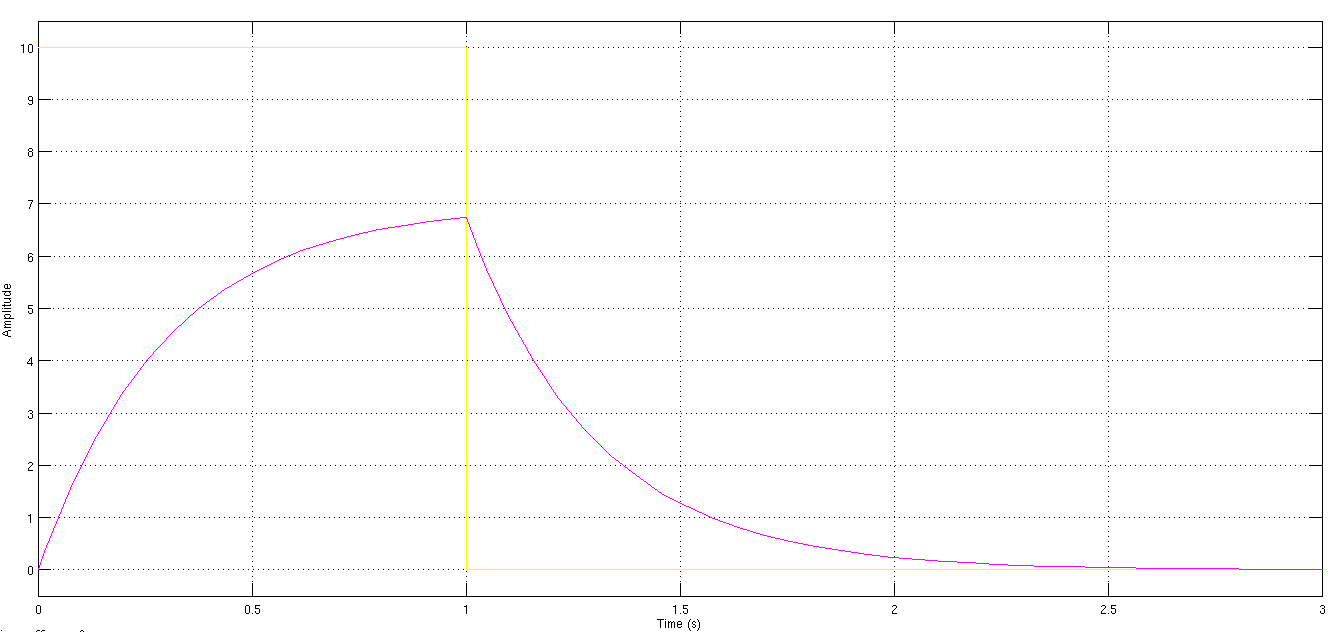
\includegraphics[scale=0.5]{figure.png}
	\caption{Simualción Punto 4, con los valores determinados.}
	\label{fig3}
\end{figure}
\noindent
La respuesta obtenida en la gráfica es la esperada, dado que es un sistema de primer orden inicia con máxima pendiente. Como la señal de entrada es la resta de $2$ pasos, pero un paso esta corrido en el tiempo después de el valor de $T=1$ esa suma de entradas es $0$, por consiguiente el calor final tendera a $0$ como se muestra en la Fig. \ref{fig1}
\end{document}